\chapter{Spin}
\section{Effetto Zeeman normale}
\paragraph{Precessione di Larmor}
Il moto circolare di una carica, come un elettrone attorno al nucleo di un atomo, è influenzato dalla presenza di un campo magnetico esterno.
In meccanica classica si nota che il momento angolare compie una precessione per effetto del campo, in un effetto noto come \emph{precessione di Larmor}.
Prendiamo la funzione lagrangiana di una particella di carica $q$ in un campo magnetico $\vec B=\rot\vec A$ uniforme,
\begin{equation}
	\lag=\frac{m}2\dot{\vec x}^2-\frac{q}{c}\scalar{\vec A}{\dot{\vec x}}.
	\label{eq:lagrangiana-campo-magnetico}
\end{equation}
In questo particolare caso è conveniente porsi nel gauge in cui $\vec A=-\frac12\vec x\times\vec B$: usando la notazione $\partial_i=\drp{}{x_i}$ abbiamo
\begin{equation}
	\begin{split}
		(\rot\vec A)_k&=\epsilon_{ijk}\partial_iA_j=-\frac12\epsilon_{ijk}\partial_i(\epsilon_{lmj}x_kB_m)=\\
		&=-\frac12\epsilon_{jki}\epsilon_{jlm}\big[(\partial_ix_l)B_m+x_l(\partial_iB_m)\big]=\\
		&=-\frac12(\delta_{kl}\delta_{im}-\delta_{km}\delta_{il})(\delta_{il}B_m+x_l\partial_iB_m)=\\
		&=-\frac12(B_k-\delta_{il}B_k+x_k\partial_iB_i-x_i\partial_iB_k)=\\
		&=-\frac12(B_k-3B_k+x_k\div\vec B-(\scalar{\vec x}{\nabla})B_k)=B_k
	\end{split}
\end{equation}
poich\'e $\div\vec B=0$ e $\vec B$ è uniforme quindi non dipende da $\vec x$: ciò mostra che, correttamente, $\rot\vec A=\vec B$.
Risulta perciò
\begin{equation}
	\lag=\frac{m}2\dot{\vec x}^2+\frac{q}{2c}\scalar{(\vec x\times\vec B)}{\dot{\vec x}}=
	\frac{m}2\dot{\vec x}^2-\frac{q}{2mc}\scalar{(\vec x\times m\dot{\vec x})}{\vec B}=
	\frac{m}2\dot{\vec x}^2-\frac{q}{2mc}\scalar{\vec L}{\vec B}.
\end{equation}
Usando le coordinate cilindriche, scegliendo l'asse verticale lungo la direzione di $\vec B$, si ha
\begin{equation}
	\lag=\frac{m}2(\dot{r}^2-r^2\dot{\phi}^2+\dot{z}^2)-\frac{q}{2c}r^2\dot{\phi}B.
\end{equation}
Il momento coniugato alla variabile angolare ora non è più solo $mr^2\dot{\phi}$, ma per l'effetto del campo magnetico si ha
\begin{equation}
	\drp{\lag}{\dot{\phi}}=mr^2\bigg(\dot{\phi}-\frac{qB}{2mc}\bigg)
\end{equation}
dove compare la cosiddetta \emph{frequenza di Larmor} $\omega_L\defeq\frac{qB}{2mc}$.
Possiamo allora cambiare il sistema di coordinate in uno ruotante attorno all'asse verticale (sempre individuato dal campo $\vec B$) con una frequenza pari a $\omega_L$, in modo da cancellare questo effetto, definendo cos\`i $\phi'\defeq \phi-\omega_Lt$.

Nella meccanica quantistica, la presenza del campo magnetico influenza anche i livelli energetici, che possiamo osservare tramite le linee spettrali di emissione: l'\emph{effetto Zeeman normale} predice che queste linee si dividono in altre tre.
Prendiamo infatti l'hamiltoniano del sistema composto da un elettrone in un atomo di idrogeno, con hamiltoniano $\op H^{(0)}$, a cui aggiungiamo il termine perturbativo (che otteniamo dalla lagrangiana della particella nella \eqref{eq:lagrangiana-campo-magnetico})\footnote{
	Il campo $\vec B$ è visto come \emph{esterno} al sistema, per cui non è quantizzato e non figura nelle prossime equazioni come operatore.
}
\begin{equation}
	\frac{e}{2mc}\scalar{\op{\vec L}}{\vec B}=-\scalar{\op{\vmu}_L}{\vec B}
	\label{eq:perturbazione-zeeman-normale}
\end{equation}
dove abbiamo definito il \emph{momento magnetico orbitale} $\op{\vmu}_L\defeq\frac{e}{2mc}\op{\vec L}$.
Consideriamo un sistema di assi cartesiani orientato in modo che l'asse $\vec e_3$ sia nella direzione di $\vec B$, e prendiamo la base solita $\ket{n,l,m_l}$, i cui numeri quantici fanno riferimento alle osservabili $\op H^{(0)}$, $\op{\vec L}^2$ e $\op L_3$.
L'hamiltoniano perturbato è cos\`i
\begin{equation}
	\op H=\op H^{(0)}+\frac{eB}{2mc}\op L_3
\end{equation}
da cui
\begin{equation}
	\op H\ket{n,l,m_l}=\bigg(E^{(0)}_n+\frac{eBm_l\hbar}{2mc}\bigg)\ket{n,l,m_l}:
\end{equation}
ciò mostra come il campo magnetico rimuove la degenerazione di $\op L_3$.
\begin{figure}
	\tikzsetnextfilename{zeeman-normale}
	\centering
	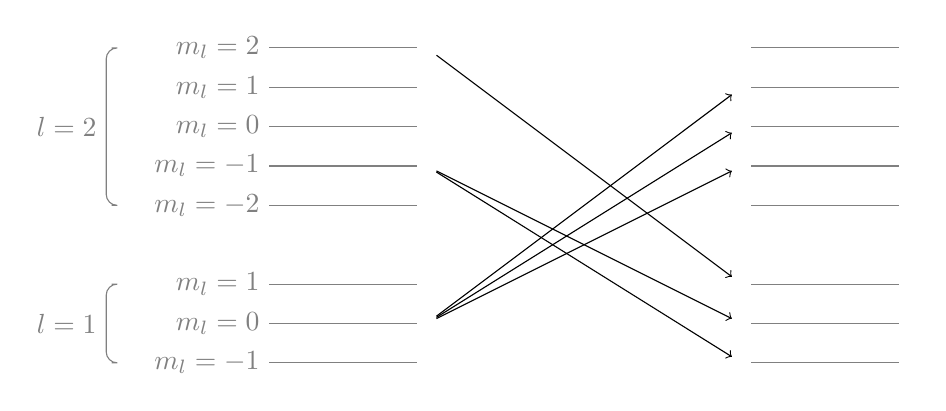
\begin{tikzpicture}
		% Sinistra
		\node (l1-1) at (-2,-1.5){};
		\node (l10)  at (-2,-1)  {};
		\node (l11)  at (-2,-0.5){};
		\node (l2-2) at (-2,0.5) {};
		\node (l2-1) at (-2,1)   {};
		\node (l20)  at (-2,1.5) {};
		\node (l21)  at (-2,2)   {};
		\node (l22)  at (-2,2.5) {};
		% Destra
		\node (r1-1) at (2,-1.5){};
		\node (r10)  at (2,-1)  {};
		\node (r11)  at (2,-0.5){};
		\node (r2-2) at (2,0.5) {};
		\node (r2-1) at (2,1)   {};
		\node (r20)  at (2,1.5) {};
		\node (r21)  at (2,2)   {};
		\node (r22)  at (2,2.5) {};
		% Raggruppamento delle linee con stesso n. quantico l
		\draw[rounded corners,black!50!white] (l1-1) ++(-4,0) -- ++(-2pt,0) to node[left]{$l=1$} ++(0,1) -- ++(2pt,0);
		\draw[rounded corners,black!50!white] (l2-2) ++(-4,0) -- ++(-2pt,0) to node[left]{$l=2$} ++(0,2) -- ++(2pt,0);
		% Linee spettrali non perturbate
		\draw[black!50!white] (l1-1) to +(-2,0) node[left]{$m_l=-1$};
		\draw[black!50!white] (l10)  to +(-2,0) node[left]{$m_l=0$};
		\draw[black!50!white] (l11)  to +(-2,0) node[left]{$m_l=1$};
		\draw[black!50!white] (l2-2) to +(-2,0) node[left]{$m_l=-2$};
		\draw[black!50!white] (l2-1) to +(-2,0) node[left]{$m_l=-1$};
		\draw[black!50!white] (l20)  to +(-2,0) node[left]{$m_l=0$};
		\draw[black!50!white] (l21)  to +(-2,0) node[left]{$m_l=1$};
		\draw[black!50!white] (l22)  to +(-2,0) node[left]{$m_l=2$};
		% Linee spettrali perturbate
		\draw[black!50!white] (r1-1) to +(2,0) node[right]{};
		\draw[black!50!white] (r10)  to +(2,0) node[right]{};
		\draw[black!50!white] (r11)  to +(2,0) node[right]{};
		\draw[black!50!white] (r2-2) to +(2,0) node[right]{};
		\draw[black!50!white] (r2-1) to +(2,0) node[right]{};
		\draw[black!50!white] (r20)  to +(2,0) node[right]{};
		\draw[black!50!white] (r21)  to +(2,0) node[right]{};
		\draw[black!50!white] (r22)  to +(2,0) node[right]{};
		% Frecce per indicare le transizioni tra i livelli
		\draw[thin,black,->] (l22) -- (r11);

		\draw[thin,black,->] (l2-1) -- (r10);
		\draw[thin,black,->] (l2-1) -- (r1-1);

		\draw[thin,black,->] (l10) -- (r21);
		\draw[thin,black,->] (l10) -- (r20);
		\draw[thin,black,->] (l10) -- (r2-1);
	\end{tikzpicture}
	\caption{Esempio della divisione di alcune linee spettrali dovuta all'effetto Zeeman normale.}
	\label{fig:zeeman-normale}
\end{figure}

Le transizioni tra livelli di energia di $\op H^{(0)}$ sono, come visto nel capitolo precedente, permesse solo se $\Delta l=\pm 1$ e $\Delta m_l=0,\pm 1$, quindi la variazione di energia tra i livelli perturbati è
\begin{equation}
	\Delta H=\Delta E^{(0)}+\frac{e\hbar B}{2mc}\Delta m_l
\end{equation}
da cui si nota che dove prima si aveva un livello, ora in corrispondenza ne osserviamo tre.
In realtà le osservazioni sperimentali mostrano che questa descrizione è sbagliata: si sono misurate più di tre linee anche non equidistanti tra loro.
Si è scoperto infatti che l'elettrone, come le altre particelle elementari, possiede un altro tipo di momento angolare, detto \emph{momento angolare intrinseco} o \emph{spin}, di cui non si è tenuto conto in queste equazioni.
